\usepackage{pgfplots}
% \pgfplotsset{width=10cm,compat=1.9}

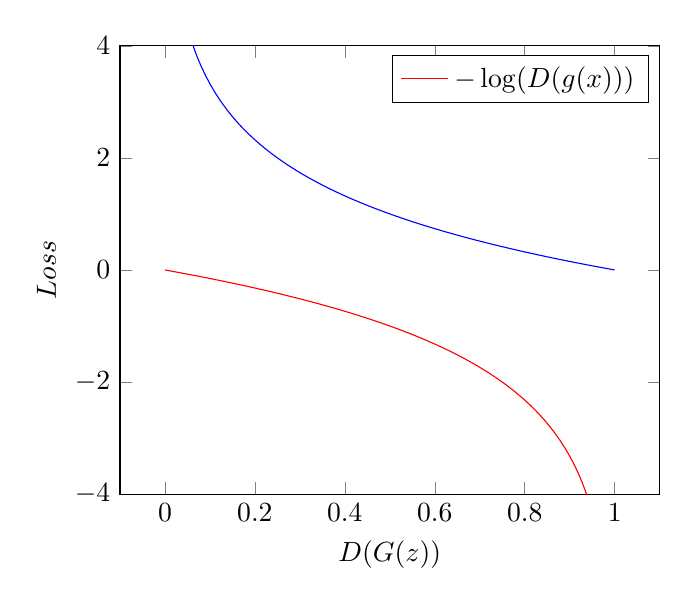
\begin{tikzpicture}
	\begin{axis}[ymin=-4,ymax=4,xlabel=$D(G(z))$,ylabel=$Loss$]
		\addplot[domain=0:1, samples=100,unbounded coords=jump,color=red]{ln(1-x)/ln(2)};
		% \addlegendentry{$\log(1-D(g(x)))$}
		\only<3->
		{
		    \addplot[domain=0:1, samples=100,unbounded coords=jump,color=blue]{-ln(x)/ln(2)};
		    \addlegendentry{$-\log(D(g(x)))$}
	    }
	\end{axis}
\end{tikzpicture}